\RequirePackage{etex}


\documentclass[11pt]{amsart}

\usepackage{minted}
\usepackage{amsfonts,amssymb,amscd,amsmath,mathrsfs,amsthm}
\usepackage{xcolor}
\usepackage{listings}
\usepackage[utf8]{inputenc}
\usepackage[english]{babel}
\usepackage{amsthm,amsmath,amsfonts,amssymb,amsbsy}
\usepackage{cite,graphicx,color,euscript,epstopdf,url,float}
\usepackage{setspace}
\usepackage{hyperref}
\usepackage{cleveref}
\usepackage{autonum}
\usepackage{caption}
\usepackage{subcaption}


% Set the margin and appearance, as set by class standards.
\setlength{\oddsidemargin}{0.25in}  %please do not change
\setlength{\evensidemargin}{0.25in} %please do not change
\setlength{\marginparwidth}{0in} %please do not change
\setlength{\marginparsep}{0in} %please do not change
\setlength{\marginparpush}{0in} %please do not change
\setlength{\topmargin}{0in} %please do not change
\setlength{\footskip}{.3in} %please do not change
\setlength{\textheight}{8.75in} %please do not change
\setlength{\textwidth}{6in} %please do not change
\setlength{\parskip}{4pt} %please do not change

% Add new functions
% Add new function for changing how the equations look
\newcommand{\crefrangeconjunction}{--}

% Change how referencing equations looks
\crefformat{equation}{(#2#1#3)}
\crefrangeformat{equation}{(#3#1#4)--(#5#2#6)}

% Use some standard appearances for math principles
\newtheorem{assumption}{Assumption}[section]
\newtheorem{definition}{Definition}[section]
\newtheorem{theorem}{Theorem}[section]
\newtheorem{lemma}{Lemma}[section]
\newtheorem{proposition}{Proposition}[section]
\newtheorem{corollary}{Corollary}[section]
\newtheorem{remark}{Remark}[section]
\newtheorem{example}{Example}[section]
\newtheorem{algorithm}{Algorithm}[section]
\newtheorem{conjecture}{Conjecture}[section]

\makeatletter
\renewcommand{\@biblabel}[1]{#1.}
\makeatother

\author{Steven~Glasford}
\title{Modeling~warring~fungi~on~a~plant.}
%Title of the first draft
%\title{Numerical Solution of a dynamic equilibrium of pathogen cohorts.}
%The following is the first title that we chose, 
%but we changed it to allow for a shorter and sleeker title.
%%%% Numerical solution of a first-order Hamilton--Jacobi equation for dynamic 
%%%% equilibrium of pathogen cohorts.

\thanks{Advisor: Dr. Ivan Yegorov}
\email{steven.glasford@ndsu.edu}
\address{Department of Mathematics, North Dakota State University, PO Box 6050,
Fargo, ND 58108-6050, USA}

\begin{document}

%The first draft of this paper is due 4 November 2020
\date{Fall~2020}

\maketitle

\begin{abstract}
    In the wild, it is widespread for fungi and other pathogens to enter plant hosts and typically result in competition from other pathogens for a single host. Also typical is when a fungus mutates, whereby natural selection or by the act of introduction into a different environment. The mutation leads to a case where the fungus that has not mutated (the resident) might have to compete with its mutated cousin.
    This paper investigates a zero-sum game between a resident and mutant strain of fungi to see if one fungus wins over the other. We also explore the case in which the two strains enter an equilibrium point where both can exist. Furthermore, this paper simulates this situation on a single plant for a single season and does not discuss the potential for evolution between seasons or the dynamics of multiple plants of the same species.
\end{abstract}


\section{Introduction}
Pathogens are what make people, pets, and every other living organism sick. They are a broad group and can do everything from making a person sick with COVID-19 to blight rotting potatoes in the field starving people. Plant pathogens are everywhere. Going outside to the park, it is not uncommon for a person to see brown spots on the leaves of trees caused by fungus or to see lichens growing on oak trees' bark. 

In this paper, a zero-sum feedback game [\ref{terms}.\ref{term:zerosum}] of two competing pathogens on a single plant, battling for dominance on the plant. To do this, we use a system of nonlinear ordinary differential equations. We use computers and numerical analysis to solve and describe the dynamics of a single growing season of two invading fungal pathogens on a single plant. 

The first fungus can be understood as the resident, while the second is the mutant. The mutant fungus is of the same species but is a different individual.  The function that describes the fungi invasion is the difference between the two marginal fitness criteria [\ref{terms}.\ref{term:marginal}], and represents the cost in defining the  differential game's value [\ref{terms}.\ref{term:differentialgame}].  A general dynamic game approach of \cite{YegorovGrognardMailleretHalkettBernhard2019} is explored and discussed. The Cauchy problem [\ref{terms}.\ref{math:cauchyproblem}] for the first-order Hamilton--Jacobi partial differential equation (HJ PDE) created by this situation is solved using the ROC-HJ software~\cite{ROCHJ2019}. 

Analysis of the numerical simulations obtained by this software package, and a graphical description is further investigated later in this document.


\section{Statement of the model}
Before we can adequately analyze the numerical solutions, we must first define the model. We consider the dynamics of two biotrophic [\ref{terms}.\ref{term:biotrohpic}] fungal cohorts [\ref{terms}.\ref{term:cohort}] on one plant in a single season.  Let us refer to them as cohorts~$ 1 $ and $ 2 $. For
cohort~$ i $, let $ n_i $ the lesion density, which is the number of mycelia [\ref{terms}.\ref{term:mycelia}]
per unit area of the host. For simplicity, assume $ n_1 $ and $ n_2 $ to be
constant during the entire infection period within the season, which means that
only the resident and the mutant exist on the plant. There are no new invaders that do not penetrate the host during the analyzed period.
In the wild, this is a substantial restriction for infections. However, it still allows us to draw significant conclusions with relevant
biological interpretations while adhering to standard experimental infection protocols.

We denote the average size of a mycelium in cohort~$ i $ by $ M_i $. Let $ S_i $
be the average quantity of spores produced by a mycelium in cohort~$ i $. The duration of the
infection~$ t $ within the season is a time variable. Note that the
mycelial sizes~$ M_1 $ and $ M_2 $ are measured in terms of equivalent amounts
of infecting spores. For instance, if a mycelium appears from one spore at the
beginning of the infection period, the initial mycelial size can be set as one or only as one spore.

To determine the nutrient flux [\ref{terms}.\ref{term:nutrientflux}]
of cohort~$ i $, we use the function,
$ f_i = f_i(M_1, M_2) $, where the flux allocation is between mycelia growth and producing spores. which is allocated between two different pathogen
activities such as within-host multiplication (mycelial growth) and producing
asexual spores. For brevity, we do not explicitly show the dependence on the
constant parameters $ n_1, n_2 $ when writing $ f_i = f_i(M_1, M_2) $,
$ i = 1,2 $. Let $ u_i = u_i(t) $ be a related resource allocation (control)
function, taking values between zero and one. 
When $ u_i(t) = 0 $, the particular fungus only produces mycelia, while when $ u_i(t) = 1 $, the fungus produces spores, and when $ 0 < u_i(t) < 1 $, the fungus is doing both to some degree.
% Suppose that the whole flux goes
% to mycelial growth when $ u_i(t) = 0 $ and to spore production when
% $ u_i(t) = 1 $, while, for $ 0 < u_i(t) < 1 $, there is an intermediate
% configuration. In other words, the fungus expends all of its energy to produce mycelia when 

Let $ g = g(M) $ be the rate of mycelial decay for both cohorts; we assume that the mutation does not. We assume a constant yield of spores, $ \delta > 0 $, as compared to mycelial growth. 

The period of the infections within the season is a fixed interval~$ [0, T] $.

The following dynamic model can thus be formulated 
\cite{YegorovGrognardMailleretHalkettBernhard2019}:
\begin{equation}
\left\{ \begin{aligned}
& \frac{\mathrm{d} M_1(t)}{\mathrm{d} t} \:\: = \:\: \left(1 - u_1(t)\right) \,
  f_1\left(M_1(t), M_2(t)\right) \: - \: g\left(M_1(t)\right), \\
& \frac{\mathrm{d} M_2(t)}{\mathrm{d} t} \:\: = \:\: \left(1 - u_2(t)\right) \,
  f_2\left(M_1(t), M_2(t)\right) \: - \: g\left(M_2(t)\right), \\
& \frac{\mathrm{d} S_1(t)}{\mathrm{d} t} \:\: = \:\: \delta \, u_1(t) \,
  f_1\left(M_1(t), M_2(t)\right), \\
& \frac{\mathrm{d} S_2(t)}{\mathrm{d} t} \:\: = \:\: \delta \, u_2(t) \,
  f_2\left(M_1(t), M_2(t)\right), \\
& M_1(0) = M_1^0, \quad M_2(0) = M_2^0, \quad S_1(0) = S_1^0,
  \quad S_2(0) = S_2^0, \\
& 0 \leqslant u_1(t) \leqslant 1, \quad 0 \leqslant u_2(t) \leqslant 1,
  \quad t \in [0, T].
\end{aligned} \right.  \label{1}
\end{equation}
Since the right-hand sides of the third and fourth equations in (\ref{1}) do
not contain $ S_1 $ and $ S_2 $, one does not need to treat $ S_1 $ and $ S_2 $
explicitly, which makes $ M_1 $ and $ M_2 $ considered only as state variables [\ref{terms}.\ref{term:statevariables}].

The reproductive success (the amount of growth on the plant) of cohort~$ i $ is determined by:
\begin{equation}
\int\limits_0^T \frac{\mathrm{d} S_i(t)}{\mathrm{d} t} \, e^{-\mu t}
    \: dt \:\: = \:\: \delta \,
\int\limits_0^T u_i(t) \, f_i\left(M_1(t), M_2(t)\right) \, e^{-\mu t} \: dt,  \label{3_1}
\end{equation}
where $ e^{-\mu t} $ describes the exponential extinction of the infections as the plant develops immunity,
and $ \mu $ is a positive constant. Since $ \delta $ is a positive constant,
we can divide \cref{3_1} by $ \delta $ and arrive at the following, where $J$ is a Jacobi function, 

\begin{equation}
J_i\left(u_1(\cdot), u_2(\cdot)\right) \:\: = \:\: \int\limits_0^T u_i(t) \, f_i\left(M_1(t),
  M_2(t)\right) \, e^{-\mu t} \: dt.  \label{3}
\end{equation}


In the next equations, we look at the zero-sum two-player differential game, in line with \cite{YegorovGrognardMailleretHalkettBernhard2019,
BernhardGrognardMailleretAkhmetzhanov2010}.
We look at the competition between the two cohorts in a single season by investigating their reproductive outputs and seeking the saddle control strategies [\ref{terms}.\ref{term:saddlecontrol}]. In other words, we try and find the point/s in which the two pathogens enter a stalemate and what actions the fungi need to do in order to enter this situation.
\begin{equation}
\left\{ \begin{aligned}
& \frac{\mathrm{d} M_1(t)}{\mathrm{d} t} \:\: = \:\: \left(1 - u_1(t)\right) \,
  f_1\left(M_1(t), M_2(t)\right) \: - \: g\left(M_1(t)\right), \\
& \frac{\mathrm{d} M_2(t)}{\mathrm{d} t} \:\: = \:\: \left(1 - u_2(t)\right) \,
  f_2\left(M_1(t), M_2(t)\right) \: - \: g\left(M_2(t)\right), \\
& M_1(0) = M_1^0, \quad M_2(0) = M_2^0, \\
& 0 \leqslant u_1(t) \leqslant 1, \quad 0 \leqslant u_2(t) \leqslant 1,
  \quad t \in [0, T],
\end{aligned} \right.  \label{7}
\end{equation}
\begin{equation}
J(u_1(\cdot), u_2(\cdot)) \:\: \longrightarrow \:\: 
\inf_{u_1(\cdot)} \:  \sup_{u_2(\cdot)} 
\:\: \mbox{or} \:\:
\sup_{u_2(\cdot)} \: \inf_{u_1(\cdot)} \, ,  \label{8}
\end{equation}
\begin{equation}
\begin{aligned}
& J\left(u_1(\cdot), u_2(\cdot)\right) \:\: = \:\: J_2\left(u_1(\cdot), u_2(\cdot)\right) \: - \:
J_1\left(u_1(\cdot), u_2(\cdot)\right) \\
& \quad
= \:\: \int\limits_0^T \left( u_2(t) \, f_2(M_1(t), M_2(t)) \: - \: u_1(t)
  \, f_1(M_1(t), M_2(t)) \right) \,
e^{-\mu t} \: dt.
\end{aligned}  \label{9}
\end{equation}
Where $\inf$ is the infimum [\ref{mathdefs}.\ref{math:infimum}] and $\sup$ is the supremum [\ref{mathdefs}.\ref{math:supremum}].


According to \cite{YegorovGrognardMailleretHalkettBernhard2019}, we represent
the nutrient fluxes [\ref{terms}.\ref{term:nutrientflux}] and decay rates as

\begin{equation}
f_i(M_1, M_2) \: = \: \nu(n_1 M_1 + n_2 M_2) \, \cdot \, \rho(M_i) \:\:\:
\forall M_1 \geqslant 0 \:\:\: \forall M_2 \geqslant 0, \quad i = 1,2, 
  \label{4}
\end{equation}
\begin{equation}
\rho(M) \: = \: \alpha \: \dfrac{M}{M + k} \quad \forall M \geqslant 0, 
  \label{5_1}
\end{equation}
\begin{equation}
\nu(n_1 M_1 + n_2 M_2) \: = \: \dfrac{1}{1 + \beta \, (n_1 M_1 + n_2 M_2)}
  \quad
\forall M_1 \geqslant 0 \quad \forall M_2 \geqslant 0,  \label{5_2}
\end{equation}
\begin{equation}
g(M) \: = \: \gamma M \quad \forall M \geqslant 0.  \label{6}
\end{equation}
$\rho$ is a positive function that specifies the flow of resources obtained by a single mycelium, and $\nu$ describes the negative consequences as the pathogens compete for resources from the single plant  \cite{YegorovGrognardMailleretHalkettBernhard2019}.

Furthermore, the following parameter values are also useful for the numerical
simulations and arise from the analysis of
\cite{YegorovGrognardMailleretHalkett2017}:
\begin{equation}
\arraycolsep=1.3pt
\def\arraystretch{1.5}
\begin{array}{c}
\alpha \: = \: 0.2 \cdot 10^4 \:\: \mathrm{spores} / \mathrm{day}, \quad
k \: = \: (1/6) \cdot 10^4 \:\: \mathrm{spores}, \\
\beta \: = \: 10^{-5} \:\: \mathrm{cm}^2 / \mathrm{spores}^2, \quad \gamma
  \: = \: 0.06 \:\: 1 / \mathrm{day}, \quad
\mu \: = \: 0.03 \:\: 1 / \mathrm{day}, \\
n_1 \: = \: 9 \:\: \mathrm{spores} / \mathrm{cm}^2, \quad n_2 \: = \: 1 \:\:
  \mathrm{spore} / \mathrm{cm}^2, \\
T \: = \: 60 \:\: \mathrm{days}.
\end{array}  \label{19}
\end{equation}

As was shown in \cite{YegorovGrognardMailleretHalkettBernhard2019}, the bounded
domain
\begin{equation}
G \:\: = \:\: \left\{ (M_1, M_2) \: \in \: \mathbb{R}^2 \: \colon \: 0 < M_1 <
  \bar{M}_1, \:
0 < M_2 < \bar{M}_2 \right\}  \label{2}
\end{equation}
with
\begin{equation}
\bar{M}_1 \: = \: \bar{M}_2 \: > \: \alpha / \gamma - k  \label{2_1}
\end{equation}
is an invariant set in the state space (if a state trajectory starts in $ G $,
it cannot leave $ G $). The parameters~$ \bar{M}_1, \bar{M}_2 $ can be
understood as 
carrying capacity [\ref{terms}.\ref{term:carryingcapacity}] estimates. 


\section{Uninvadable and evolutionarily stable strategies}
In war, there are times in which neither party wins. Where there is a boundary or other concessions exist, the resident is uninvadable under this circumstance. This section describes the strategies and functions used to model a stable and uninvadable resident pathogen. In other words, we see where the two pathogens enter a stalemate, and we look deeper at the game-theoretic statements from {\rm \cref{7,8,9}}.

Based on the terminology of Adaptive Dynamics \cite{DercoleRinaldi2008}, let
us interpret cohort~{\rm 1} as a resident and cohort~{\rm 2} as a mutant.
Denote the corresponding classes of considered strategies as $ \mathcal{U}_1 $
and $ \mathcal{U}_2 $. For a pair of methods
$ \: (u_1, u_2) \, \in \, \mathcal{U}_1 \times \mathcal{U}_2, \: $
the resident is not invaded by the mutant if and only if
$$
J(u_1, u_2) \: = \: J_2(u_1, u_2) - J_1(u_1, u_2) \: \leqslant \: 0.
$$
A strategy 
$ \hat{u}_1 \in \mathcal{U}_1 $
is hence uninvadable, and the winner of the war is the resident if and only if
$$
J \left( \hat{u}_1, u_2 \right) \: \leqslant \: 0 \quad \forall u_2 \in
  \mathcal{U}_2,
$$
which is equivalent to
$$
\sup_{u_2 \, \in \, \mathcal{U}_2} \: J \left( \hat{u}_1, u_2 \right) \:\:
  \leqslant \:\: 0
$$
where $\sup$ is the supremum [\ref{mathdefs}.\ref{math:supremum}].


Such a $ \hat{u}_1 $ exists if
\begin{equation}
\inf_{u_1 \, \in \, \mathcal{U}_1} \: \sup_{u_2 \, \in \, \mathcal{U}_2} \:
  J(u_1, u_2) \:\: = \:\:
\min_{u_1 \, \in \, \mathcal{U}_1} \: \sup_{u_2 \, \in \, \mathcal{U}_2} \:
  J(u_1, u_2) \:\: \leqslant \:\: 0  \label{9_2}
\end{equation}
or
\begin{equation}
\inf_{u_1 \, \in \, \mathcal{U}_1} \: \sup_{u_2 \, \in \, \mathcal{U}_2} \:
  J(u_1, u_2) \:\: < \:\: 0  \label{9_4}
\end{equation}
(The latter inequality arises from when the infimum [\ref{mathdefs}.\ref{math:infimum}] $u_1$ is not satisfied).
Equation \cref{9_2} motivates our game-theoretic statement~{\rm \cref{7,8,9},}
where the first player tries to maximize its resistance to an invasion by the
second one{\rm ,} and vice versa. In other words, the resident fungus tries to grow and fight the opposing mutant fungus, and the mutant fungus tries to do the same.

If $ M_1^0 = M_2^0 $ and $ \mathcal{U}_1 = \mathcal{U}_2 = \mathcal{U} ${\rm ,}
then $ J(u, u) = 0 $ for all $ u \in \mathcal{U} ${\rm ,} and {\rm (\ref{9_2})}
simplifies to
\begin{equation}
\min_{u_1 \, \in \, \mathcal{U}} \: \sup_{u_2 \, \in \, \mathcal{U}} \:
  J(u_1, u_2) \:\: = \:\: 0  \label{9_3}
\end{equation}
This equation is the boundary where neither the resident and the mutant win, and there is a stalemate.
In this case{\rm ,} a strategy
$$
\hat{u}_1 \:\: \in \:\: \mathrm{Arg} \min_{u_1 \, \in \, \mathcal{U}}
  \left( \sup_{u_2 \, \in \, \mathcal{U}} \: J(u_1, u_2) \right)
$$
where $\mathrm{Arg} \min$ is the argument of the minimum [\ref{mathdefs}.\ref{math:Argmaxmin}]. The strategy is called evolutionary stable, and there is a boundary where neither pathogen wins if the related maximum for $ u_2 $ is
unique:
$$
\mathrm{Arg} \max_{u_2 \, \in \, \mathcal{U}} \: J \left( \hat{u}_1, u_2
  \right) \:\: = \:\: \left\{ \hat{u}_1 \right\}.
$$
where $\mathrm{Arg}\max$ is the argument of the maximum [\ref{mathdefs}.\ref{math:Argmaxmin}].


This approach to defining stable evolutionary strategies was initially proposed
in \cite{BernhardGrognardMailleretAkhmetzhanov2010} and further developed
in \cite{YegorovGrognardMailleretHalkettBernhard2019}.


\section{Hamilton--Jacobi--Isaacs equation}
To determine how evolutionary strategies change over time, we must develop a system of differential functions. This circumstance can be solved using a Hamilton--Jacobi-Isaacs equation. We exclude the reasoning behind using this for brevity, \cite{YegorovGrognardMailleretHalkettBernhard2019} contains more information and further analysis.

We introduce the following function known as Hamiltonian:
\begin{equation}
\begin{aligned}
& H(t, M_1, M_2, u_1, u_2, p_1, p_2) \:\: = \:\:
p_1 \, \left((1 - u_1) \, f_1(M_1, M_2) \: - \: g(M_1)\right) \\
& \qquad\qquad\qquad\qquad\qquad\quad \:\:\:\,
+ \:\: p_2 \, \left((1 - u_2) \, f_2(M_1, M_2) \: - \: g(M_2)\right) \\
& \qquad\qquad\qquad\qquad\qquad\quad \:\:\:\,
+ \:\: e^{-\mu t} \, (u_2 \, f_2(M_1, M_2) \: - \: u_1 \, f_1(M_1, M_2)) \\
& \forall t \in [0, T] \quad \forall \: (M_1, M_2) \: \in \: G \quad \forall
  \: (u_1, u_2) \: \in \: [0, 1]^2 \quad
\forall \: (p_1, p_2) \: \in \: \mathbb{R}^2
\end{aligned}  \label{12}
\end{equation}
(this is the sum of the dot product of $ \: p = (p_1, p_2) \: $ with
$ \: (\mathrm{d} M_1 / \mathrm{d} t, \, \mathrm{d} M_1 / \mathrm{d} t) \: $ and
the integrand in $ \: J(u_1(\cdot), u_2(\cdot)), \: $ see \cref{7} and
%%%%%%%%%%%%%%%%%%%%%%%%%%%
\cref{9}). The Hamiltonian satisfies the saddle point condition [\ref{mathdefs}.\ref{math:saddlepoint}] concerning
the control variables~$ u_1 $ and
$ u_2 $
\begin{equation}
\begin{aligned}
& \min_{u_1 \in [0, 1]} \: \max_{u_2 \in [0, 1]} \: H(t, M_1, M_2, u_1, u_2,
  p_1, p_2) \\
& \qquad
= \:\: \max_{u_2 \in [0, 1]} \: \min_{u_1 \in [0, 1]} \: H(t, M_1, M_2, u_1,
  u_2, p_1, p_2) \:\:
= \:\: \mathcal{H} (t, M_1, M_2, p_1, p_2) \\
& \forall t \in [0, T] \quad \forall \: (M_1, M_2) \: \in \: G \quad \forall
  \: (p_1, p_2) \: \in \: \mathbb{R}^2
\end{aligned}  \label{13}
\end{equation}
(here minimax and maximin [\ref{mathdefs}.\ref{math:maximinminimax}] give the same result). Due to the theoretical
results of \cite[\S XI.6]{FlemingSoner2006}, the value function 
$ \: V \colon [0, T] \times G \to \mathbb{R} \: $ in the formulated feedback
differential game is a unique solution of the following Cauchy problem [\ref{mathdefs}.\ref{math:cauchyproblem}] for the
Hamilton--Jacobi--Isaacs partial differential equation (HJI PDE):
\begin{equation}
\left\{ \begin{aligned}
& \frac{\partial V(t, M_1, M_2)}{\partial t} \: + \: \mathcal{H}
  \left( t, M_1, M_2, \frac{\partial V(t, M_1, M_2)}{\partial M_1},
  \frac{\partial V(t, M_1, M_2)}{\partial M_2} \right) \:\: = \:\: 0, \\
& V(T, M_1, M_2) \: = \: 0, \\
& t \in [0, T], \quad (M_1, M_2) \: \in \: G.
\end{aligned} \right.  \label{15}
\end{equation}

In general, the solution may be 
nonsmooth [\ref{mathdefs}.\ref{math:nonsmooth}] and understood in a generalized (viscosity [\ref{mathdefs}.\ref{math:viscosity}] or minimax) sense \cite{FlemingSoner2006,Subbotin1995}. These conditions make it difficult, if not impossible, to find an exact solution.

The general properties of value functions of zero-sum feedback
differential games \cite{BotkinHoffmannTurova2011} limit how fast the value function~$ V $ changes. These limitations make it Lipschitz continuous [\ref{mathdefs}.\ref{math:lipschitz}] in $ [0, T] \times G $. 
Rademacher's theorem [\ref{mathdefs}.\ref{math:rademacher}]
is differentiable almost everywhere in $ (0, T) \times G $, except
for possibly a 
subset of Lebesgue measure zero. 

For points~$ (t, M_1, M_2) $ at which the value function is differentiable,
one can obtain the saddle feedback control strategies (where the fungi enter a stalemate) from the relations
$$
\begin{aligned}
& u_1(t, M_1, M_2) \:\: \in \:\: \mathrm{Arg} \min_{w_1 \in [0, 1]}
  \left\{ \max_{w_2 \in [0, 1]} \:
H \left( t, M_1, M_2, w_1, w_2, {}^{{}^{{}^{{}^{{}^{}}}}} \right. \right. \\
& \qquad\qquad\qquad\qquad\qquad\qquad\qquad\qquad\qquad
\left. \left. \frac{\partial V(t, M_1, M_2)}{\partial M_1}, \,
  \frac{\partial V(t, M_1, M_2)}{\partial M_2} \right) \right\}, \\
& u_2(t, M_1, M_2) \:\: \in \:\: \mathrm{Arg} \max_{w_2 \in [0, 1]}
  \left\{ \min_{w_1 \in [0, 1]} \:
H \left( t, M_1, M_2, w_1, w_2, {}^{{}^{{}^{{}^{{}^{}}}}} \right. \right. \\
& \qquad\qquad\qquad\qquad\qquad\qquad\qquad\qquad\qquad
\left. \left. \frac{\partial V(t, M_1, M_2)}{\partial M_1}, \,
  \frac{\partial V(t, M_1, M_2)}{\partial M_2} \right) \right\},
\end{aligned}
$$
which reduce to
\begin{equation}
\begin{aligned}
& u_1(t, M_1, M_2) \:\: = \:\: \begin{cases}
0, & e^{-\mu t} \: + \: \frac{\partial V(t, M_1, M_2)}{\partial M_1}
  \: < \: 0, \\
1, & e^{-\mu t} \: + \: \frac{\partial V(t, M_1, M_2)}{\partial M_1}
  \: > \: 0, \\
\mbox{arbitrary from} \:\: [0, 1], & e^{-\mu t} \: + \: \frac{\partial
  V(t, M_1, M_2)}{\partial M_1} \: = \: 0,
\end{cases} \\
& u_2(t, M_1, M_2) \:\: = \:\: \begin{cases}
0, & e^{-\mu t} \: - \: \frac{\partial V(t, M_1, M_2)}{\partial M_2}
  \: < \: 0, \\
1, & e^{-\mu t} \: - \: \frac{\partial V(t, M_1, M_2)}{\partial M_2}
  \: > \: 0, \\
\mbox{arbitrary from} \:\: [0, 1], & e^{-\mu t} \: - \: \frac{\partial V(t,
M_1, M_2)}{\partial M_2} \: = \: 0.
\end{cases}
\end{aligned}  \label{16}
\end{equation}
These are resource allocation strategies and functions that describe the equilibrium point and the cohorts coexisting. In other words, these equations describe the points where the two fungi enter a stalemate dynamically as time progresses. 



\section{Numerical solution}
As described previously, these equations are complicated to solve exactly. luckily, we do not necessarily need an exact answer. Numerical analysis is the math behind finding such answers from challenging problems. In our case, there is already a program to solve Hamilton--Jacobi equations called ROC-HJ \cite{ROCHJ2019}. It is written in C++ and allows for a fast and easy
transcription of the functions above into machine code. 

Most of the preconfigured files and procedures of ROC-HJ allow for a quick transcription
of a Hamilton-Jacobi equation. \cite{ROCHJ2019} provides more information about how to install ROC-HJ, including further documentation.To use ROC-HJ, we must assign a few variables to describe the kind
of problem. Fig. \ref{code:defaults} contains some of the variables which
describe the problem. We also need to specify both a cost function (fig. \ref{code:cost}) and a dynamic equation (fig. \ref{code:dynamic}) to produce the data that we need.


Within the \texttt{data\_*.h} file, there is much more information describing
the function. One can find more information and details about this project's
configuration variables by directly viewing the data file \cite{data_ivan.h}.

In converting these equations into machine code, we must consider the Cauchy problem~\cref{15} for the HJI PDE with the nutrient
fluxes~\cref{4,5_1,5_2}, decay rate~\cref{6}, and parameter values~\cref{19}. We must further set the software to finding the solutions using a finite difference method 
\cite{FlemingSoner2006,
      OsherShu1991,
      BotkinHoffmannTurova2011,
      BokanForcadelZidani2010}
using the ROC-HJ software~\cite{ROCHJ2019}. One can find these ``default'' parameters in figure \ref{code:defaults}.

For practical purposes with ROC-HJ, it is reasonable to rewrite \cref{15} in reverse
time $ \tau = T - t $ as
\begin{equation}
\left\{ \begin{aligned}
& \frac{\partial V(T - \tau, M_1, M_2)}{\partial \tau} \:\: + \:\:
\max_{u_1 \in [0, 1]} \: \min_{u_2 \in [0, 1]} \:
\left( -H \left( T - \tau, \, M_1, \, M_2, \, u_1, \, u_2, 
{}^{{}^{{}^{{}^{{}^{}}}}} \right. \right. \\
& \qquad\qquad\qquad\qquad\qquad
\left. \left. \frac{\partial V(T - \tau, M_1, M_2)}{\partial M_1}, \,
\frac{\partial V(T - \tau, M_1, M_2)}{\partial M_2} \right) \right) \:\: =
\:\: 0, \\
& V(T - \tau, M_1, M_2) \left|_{\tau = 0} \right. \: = \: 0, \\
& \tau \in [0, T], \quad (M_1, M_2) \: \in \: G,
\end{aligned} \right.  \label{75}
\end{equation}
and then to rewrite (\ref{75}) in the new normalized state variables
\begin{equation}
m_i \, = \, M_i \cdot 10^{-4}, \quad i = 1,2  \label{75_1}
\end{equation}
(such changes of the time and state variables lead to an equivalent problem).


We specify the carrying capacity estimates as $ \: \bar{M}_1 = \bar{M}_2 =
\bar{M} = 3.5 \cdot 10^4 $,
$ \: \bar{m} = \bar{M} \cdot 10^{-4} = 3.5 \cdot 10^{-4}, \: $ and 
discretize the computational region (how much the computer will increase its measurements after each pass)
$$
\left\{ (m_1, m_2, \tau) \: \colon \: 0 \leqslant m_1 \leqslant \bar{m}, \:\: 0
\leqslant m_2 \leqslant \bar{m}, \:\:
0 \leqslant \tau \leqslant T \right\}
$$
by the spatial step $ \: \Delta m_1 = \Delta m_2 = \Delta m = 2 \cdot 10^{-3}
\: $ and time step $ \Delta \tau = 5 \cdot 10^{-3} $.

Monotone [\ref{mathdefs}.\ref{math:monotone}] finite difference methods, where there is a strictly increasing or decreasing behavior.
%%This is not very useful since the system is not solved using this method, as it is too slow
%(including the classical Lax--Friedrichs scheme)
These methods ensure theoretical convergence properties (properties where an increase in computational expenditure increases precision) with error estimates. However, they are mostly of the first order. They may generate so-called 
numerical diffusion problems [\ref{mathdefs}.\ref{math:diffusionproblem}]
on long time intervals. One way to reduce and eliminate such practical issues is to use 
higher-order ENO (essentially non-oscillatory) schemes 
such as those initially proposed \cite{OsherShu1991}. Higher-order ENO schemes also have been shown to have a more significant amount of stability, which is useful in eliminating practical issues. They are not necessarily
monotone. There is a lack of associated convergence theorems, meaning it is challenging to ensure that the computation will approach a steady answer. However,
their relevance is justifiable by various numerical experiments 
\cite{OsherShu1991,BokanForcadelZidani2010}.

We have used the second-order ENO scheme in ROC-HJ (fig.~\ref{code:defaults}) to approximate the partial
derivatives concerning the state variables, coupled with the 
second-order Runge--Kutta time discretization scheme. Runge--Kutta provides provides increased accuracy over other methods of discretely partitioning time intervals \cite{ROCHJ2019}.
To evaluate the partial derivatives $ \partial V / \partial M_i $, $ i = 1,2 $,
in the saddle feedback control representations~\cref{16}, we have applied the
standard second-order symmetrized approximation
\cite[\S 5.7]{PressTeukolskyVetterlingFlannery2007}.

Figs.~\ref{Fig_4} and \ref{Fig_5} show the reductions of the approximate
value function and corresponding saddle feedback control strategies to the
coordinate plane $ (m_1, m_2) $ for the time instants 
$ \tau = 0 $ ($ t = T = 60 $), $ \tau = 5 $ ($ t = T - 5 = 55 $),
$ \tau = \tau^{**} 
\approx 11.175 $ ($ t = T - \tau^{**} \approx 48.825 $),
and $ \tau = T = 60 $ ($ t = 0 $). 


Figure \ref{fig_4_d} shows the ``beginning'' of the simulation, where competitive strategies have not developed. There is plenty of space and resources for both of the fungi. However, sharper edges appear as the fungi begin to either produce mycelia or produce spores. After the initial production, there is a leveling off as the fungi begin conducting spore and mycelia growth simultaneously.

Figure \ref{fig_4_c} shows that at the time point of $t=48.825$, there is more differentiation in the fungi's actions where the fungi try and compete, as there is an attempt to try and stay in the battle. Figure \ref{fig_4_b} shows that the competition increases much more near the end of the simulation. The slope becomes more pronounced as the competitive forces begin to increase.

Figure \ref{fig_4_a} shows the end of the simulation, where $t=60$. The graph is flat as there are no more resources that the fungi can expend (as it is the end of the simulation). If the simulation were allowed to continue, it would continue to grow, and the slope would most likely be more pronounced than in \ref{fig_4_b}. 

In figure \ref{Fig_4}, there is no clearly defined winner. This model focuses on the efforts of the fungi attempting to remain at equilibrium. However, if the resident does not attempt to remain at equilibrium, it will be invaded and eliminated.


% Fig.~\ref{Fig_4} determines which part of the fungus that needs to advance in order to have a stalemate with the other fungus. For example, in figure \ref{Fig_4}.\ref{fig_4_a}, there has not developed a need for either fungi to try and compete with each other, this means that there is enough resources for the two of them to coexist peacefully. This is in contrast to figure \ref{Fig_4}.\ref{fig_4_b} that shows more competition occurring between the resident $m_1$ and the mutant $m_2$, and when the resident produces more mycelia there is a lack of room for the mutant to grow its mycelia and it responds with an increase in the production of spores. 

% Figure \ref{Fig_4}.\ref{fig_4_c} shows that a particular time ($t=48.825$) the particular strategies that the fungi are taking in order to enter equilibrium, again the dynamics are similar to \ref{Fig_4}.\ref{fig_4_b} where if $m_1=1$ then the resident will be expending its energy for the production of spores, and if it is zero then it is expending all of its energy producing mycelia. 
 
% Here $ \tau^{**} $ is the reverse time instant
% that triggers the appearance of singular control regimes and is obtained
% together with the equilibrium steady state~$ \left( M^{**}, M^{**} \right) $
% from the analysis based on 
% Pontryagin's principle [\ref{mathdefs}.\ref{math:pontryagin}] 
% \cite{YegorovGrognardMailleretHalkettBernhard2019}. Note that Pontryagin's
% principle for zero-sum two-player differential games describes necessary
% conditions for saddle open-loop strategies \cite{Yong2015}.

\begin{figure}
    % \centering
    \begin{subfigure}{.48 \textwidth}
        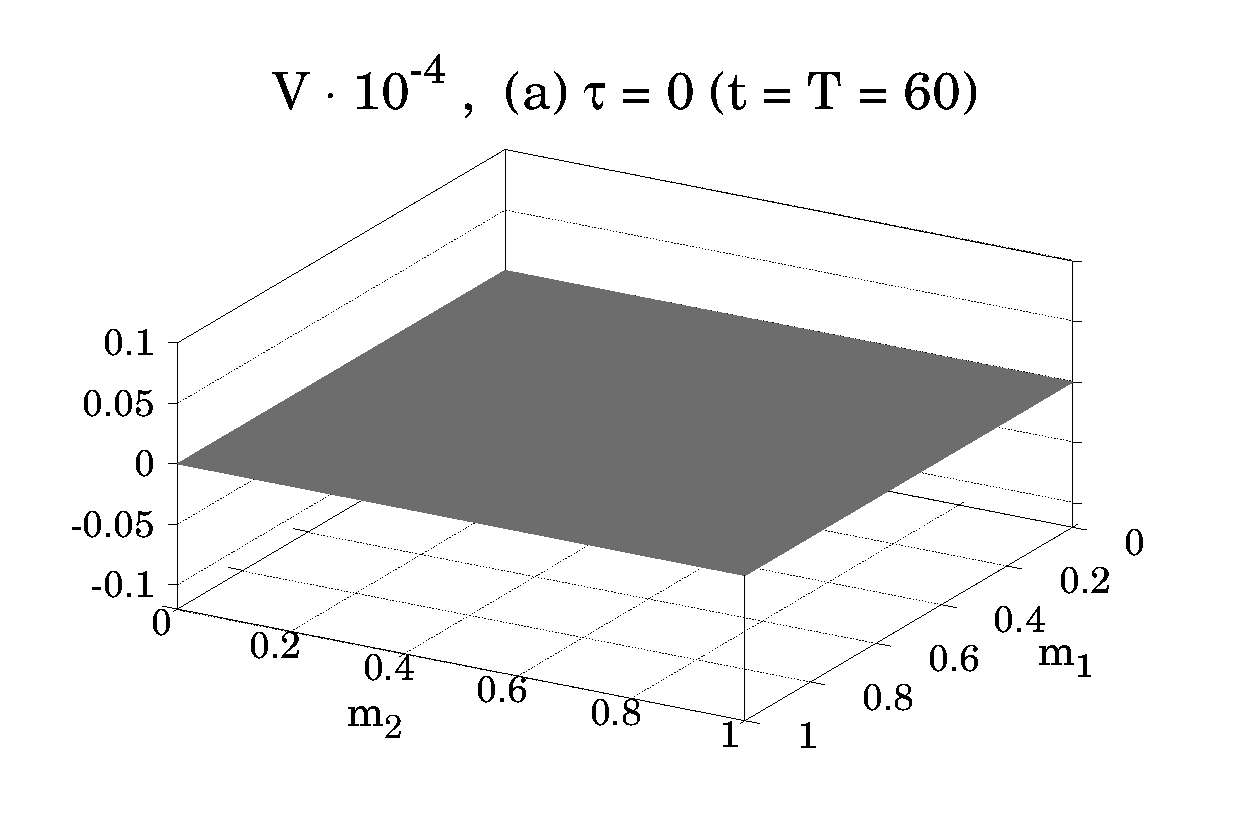
\includegraphics[width = \textwidth]{figures/Figure_4a.pdf}
        \caption{Strategies conducted at the end of the simulation.}
        \label{fig_4_a}
    \end{subfigure}
    \hfill
    \begin{subfigure}{.48 \textwidth}
        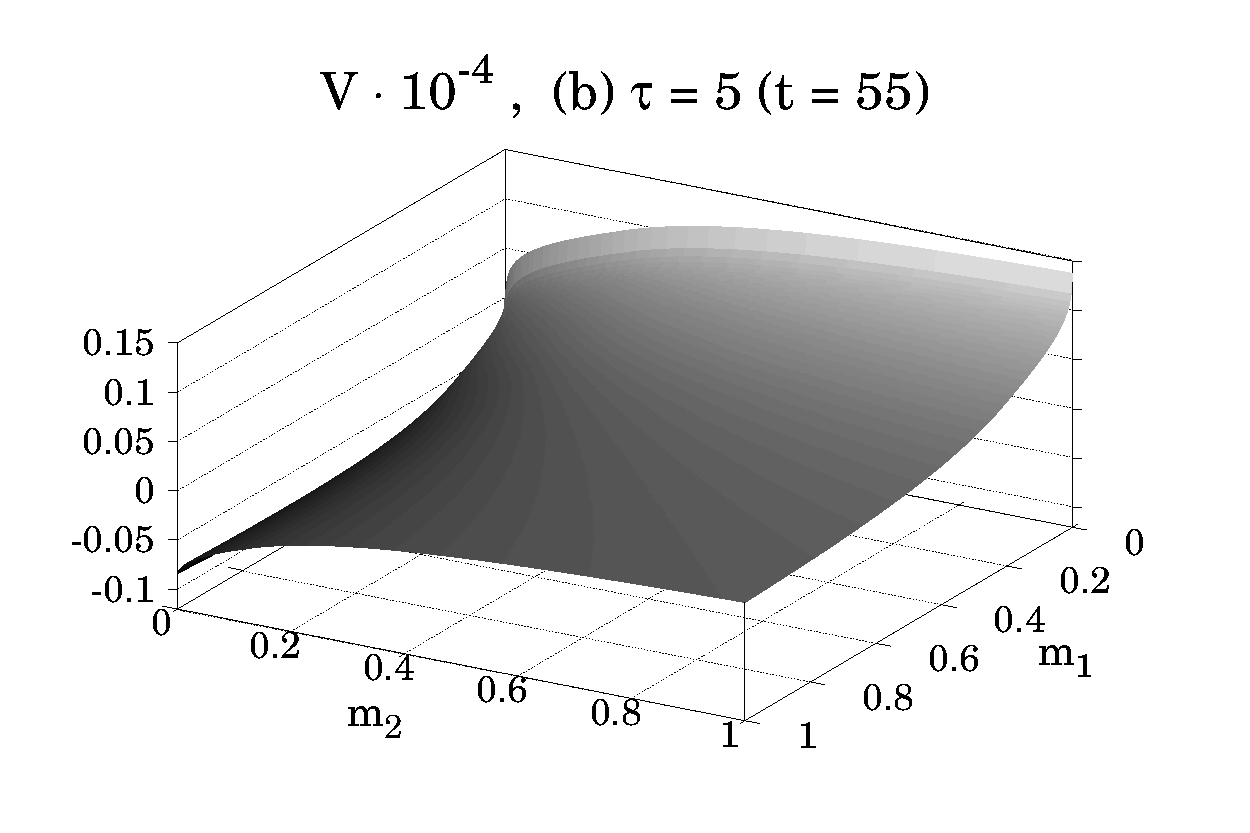
\includegraphics[width = \textwidth]{figures/Figure_4b_1.pdf}
        \caption{Competition between the fungi increases near the end of the simulation.}
        \label{fig_4_b}
    \end{subfigure}
    \hfill
    \begin{subfigure}{.48 \textwidth}
        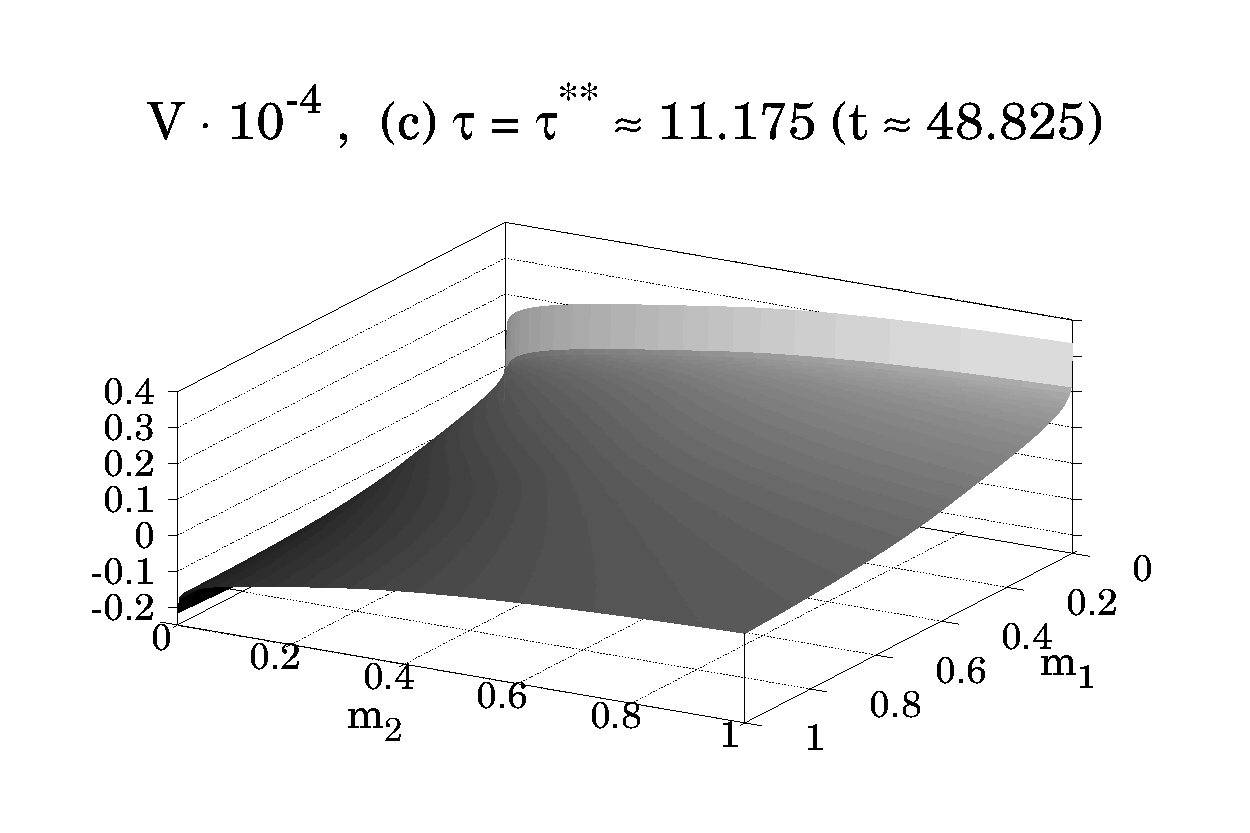
\includegraphics[width = \textwidth]{figures/Figure_4c_1.pdf}
        \caption{Competition and strategies begin to evolve.}
        \label{fig_4_c}
    \end{subfigure}
    \hfill
    \begin{subfigure}{.48 \textwidth}
        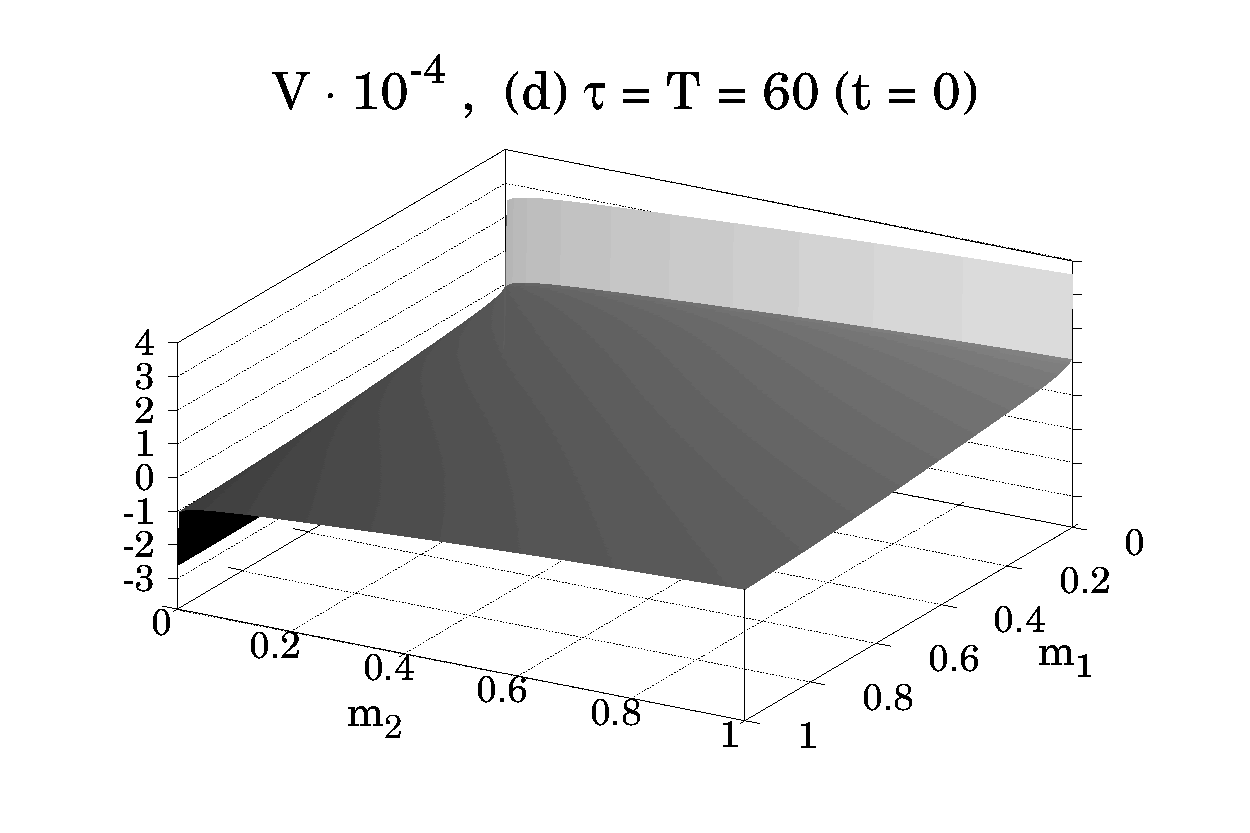
\includegraphics[width = \textwidth]{figures/Figure_4d_1.pdf}
        \caption{Strategies begin to form as the fungi take their first move.}
        \label{fig_4_d}
    \end{subfigure}

\bf \caption{\it The time instants are in reverse order to show how the computer computes the strategies using reverse time meaning the first graph is the last computation.}
\label{Fig_4}
\end{figure}


\begin{figure}
\center{ 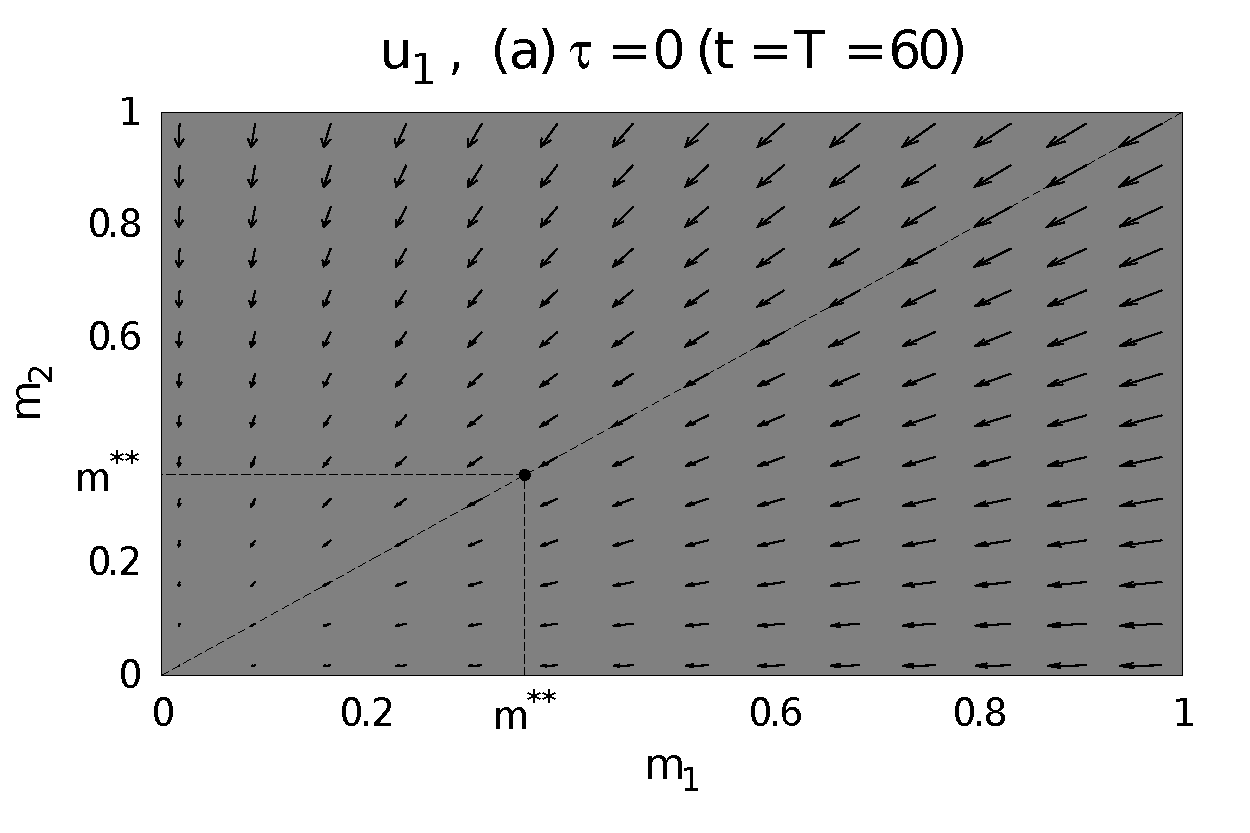
\includegraphics[width = 0.48 \textwidth]{figures/Figure_5a_1.pdf}
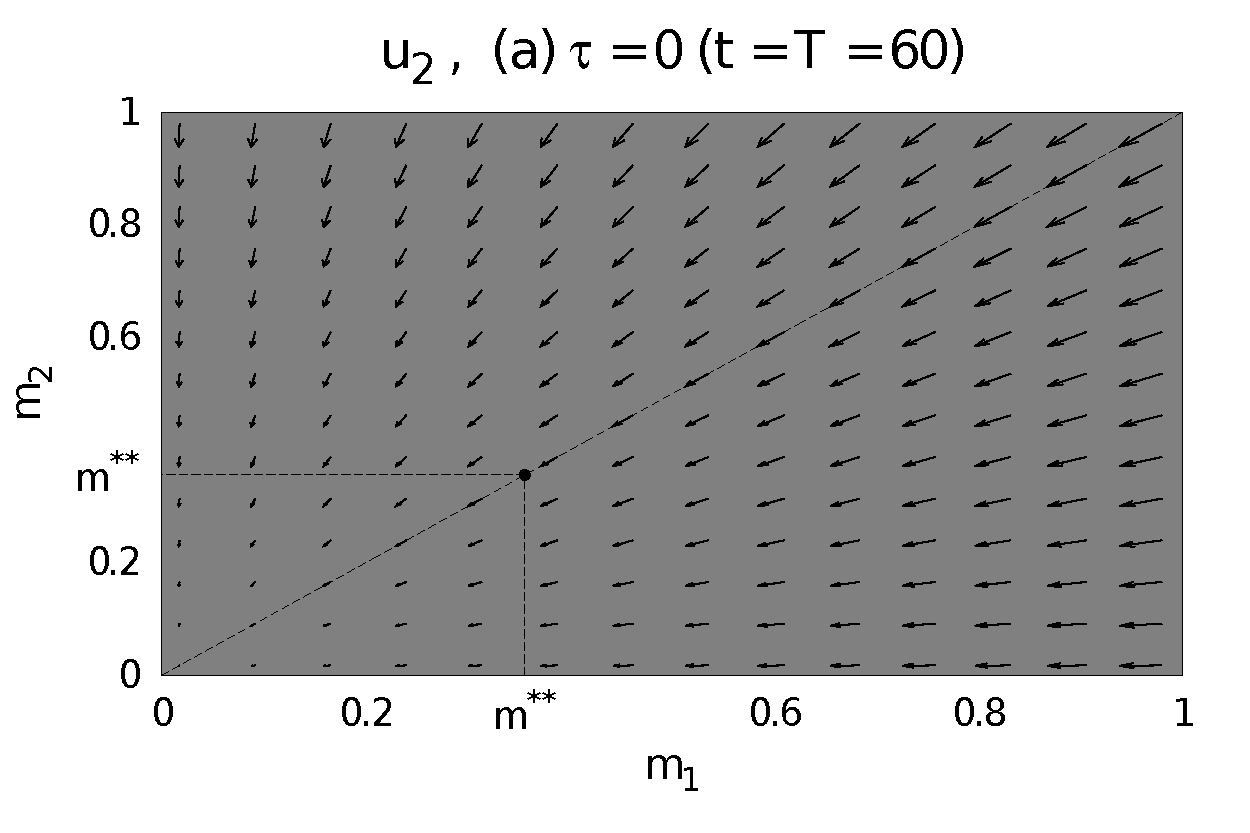
\includegraphics[width = 0.48 \textwidth]{figures/Figure_5a_2.pdf} \\
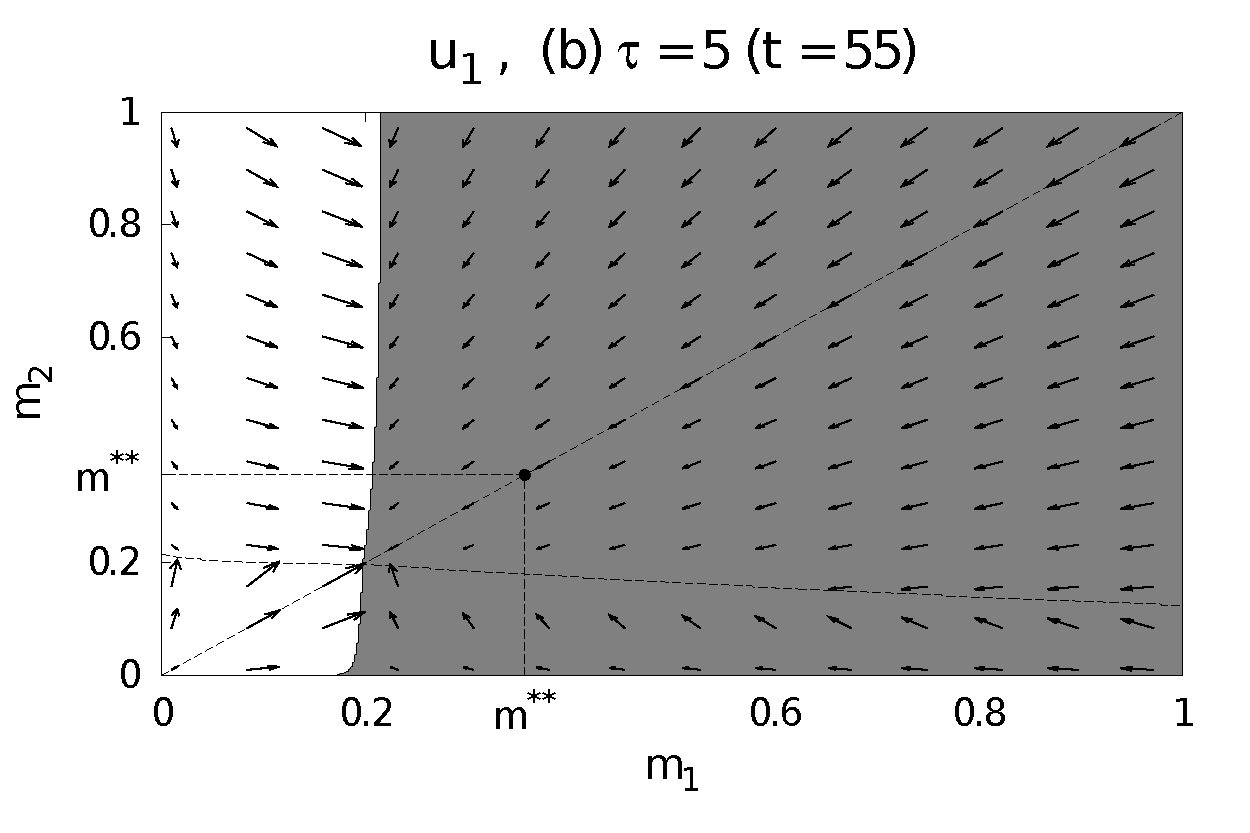
\includegraphics[width = 0.48 \textwidth]{figures/Figure_5b_1.pdf}
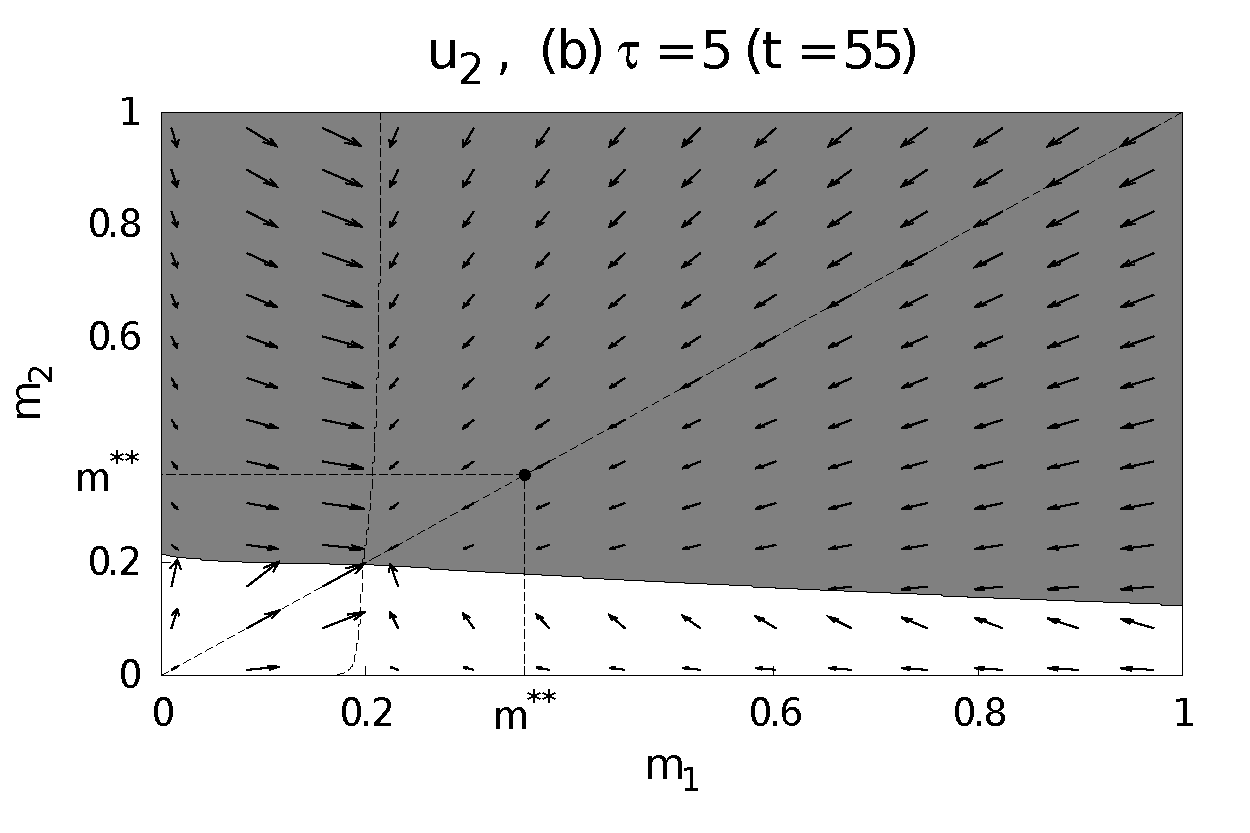
\includegraphics[width = 0.48 \textwidth]{figures/Figure_5b_2.pdf} \\
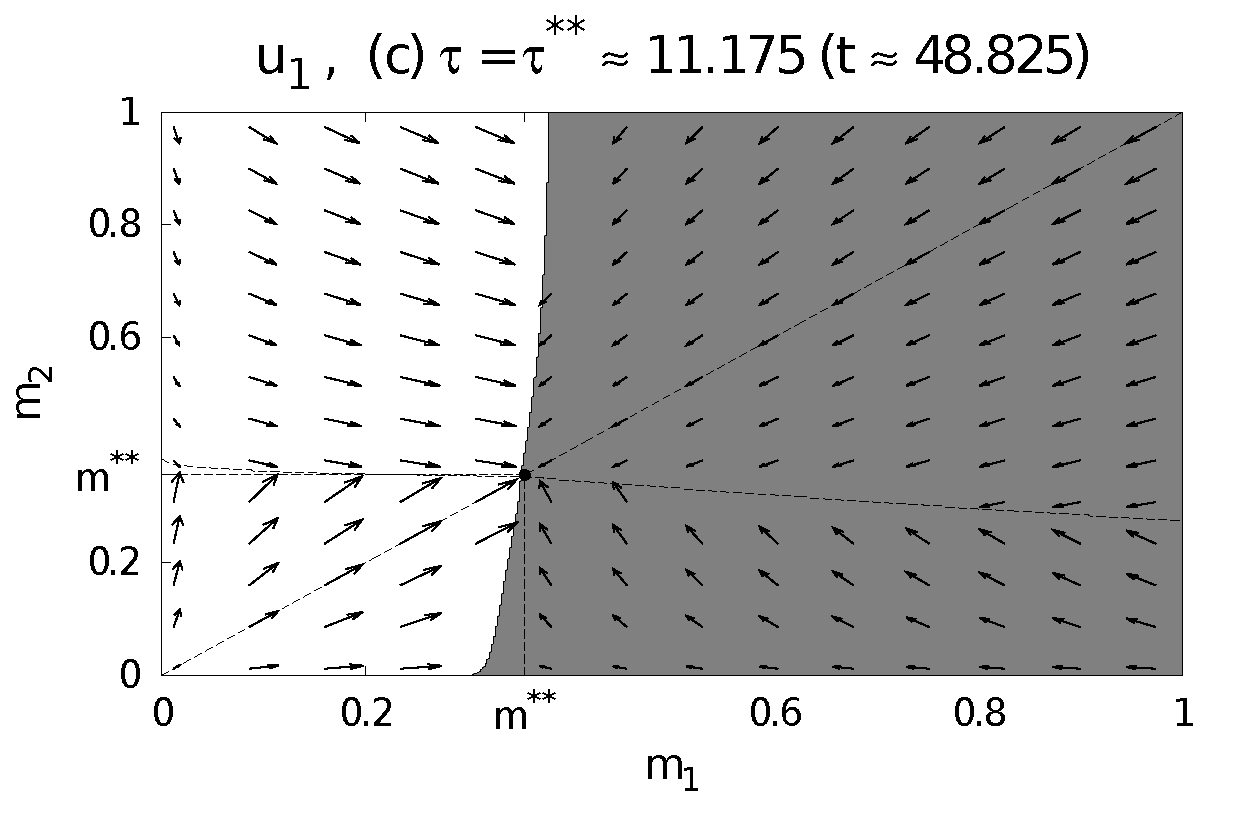
\includegraphics[width = 0.48 \textwidth]{figures/Figure_5c_1.pdf}
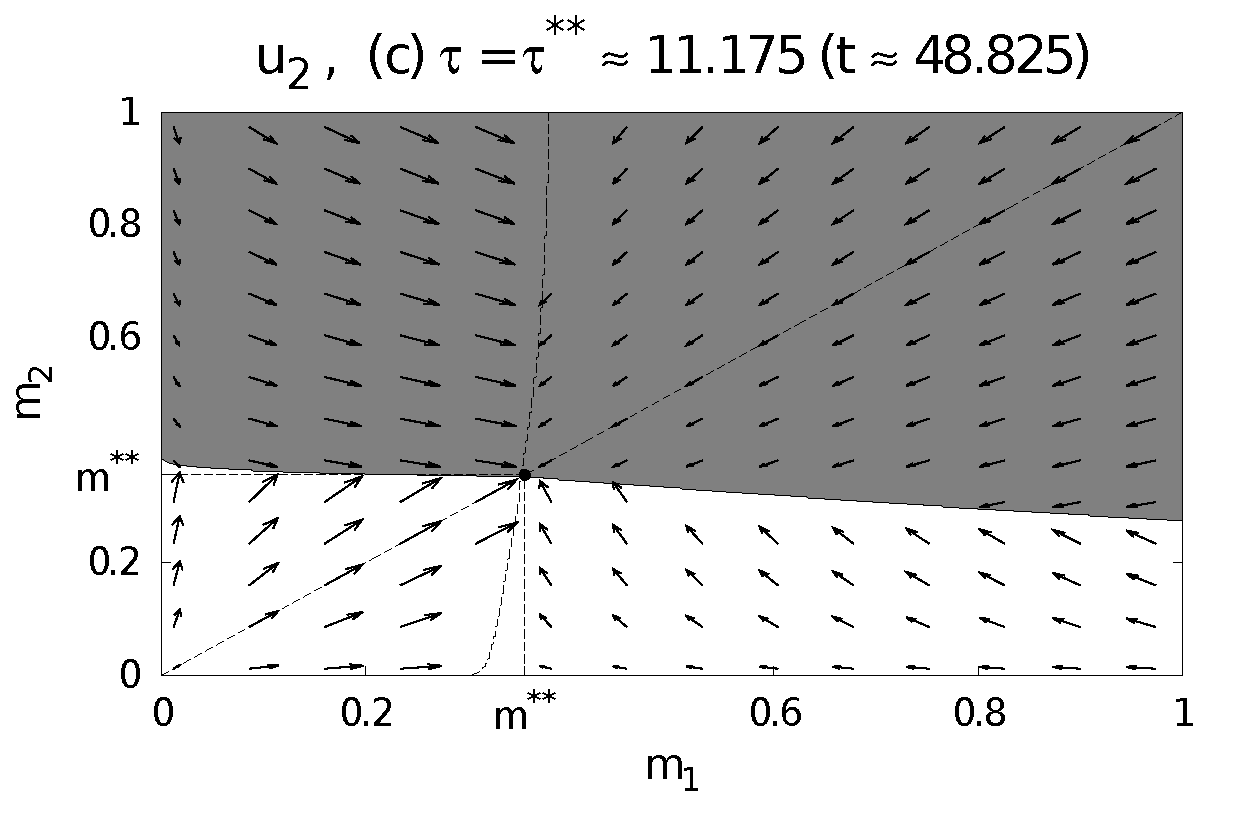
\includegraphics[width = 0.48 \textwidth]{figures/Figure_5c_2.pdf} \\
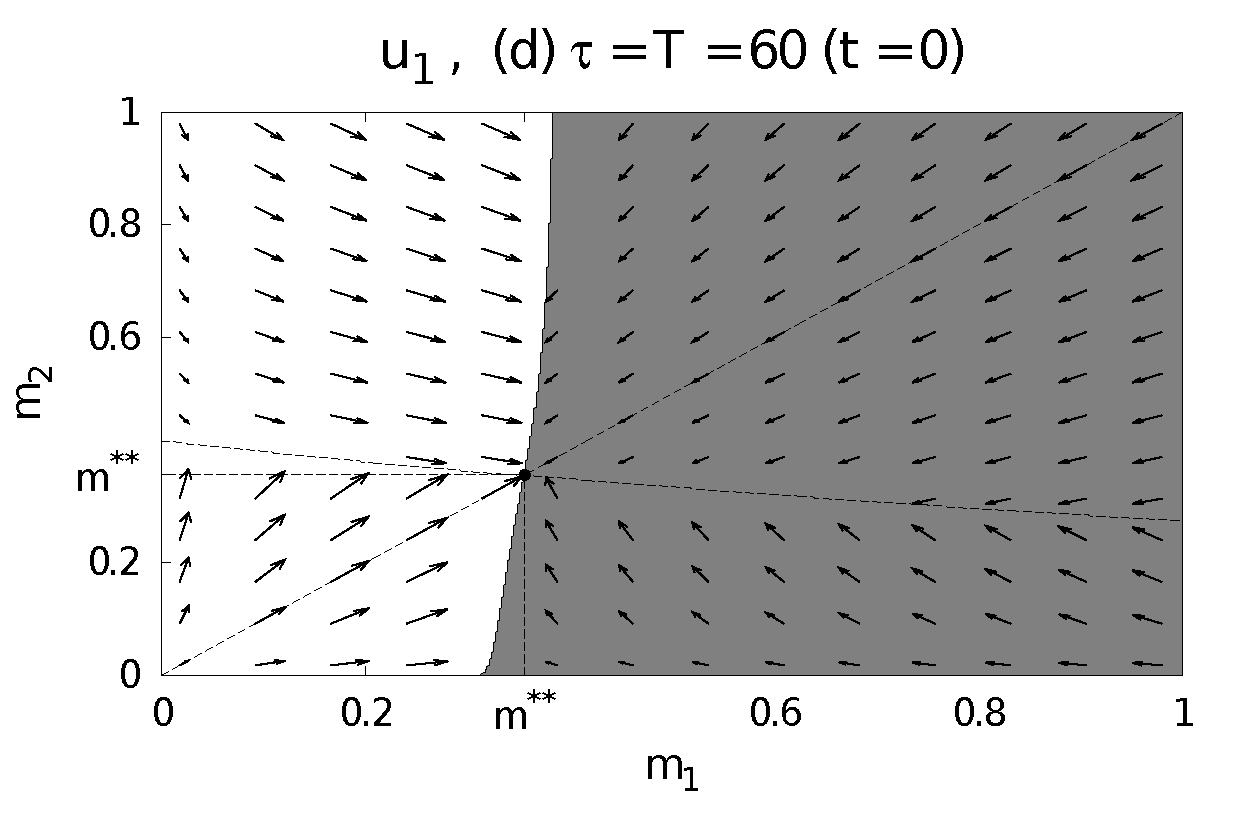
\includegraphics[width = 0.48 \textwidth]{figures/Figure_5d_1.pdf}
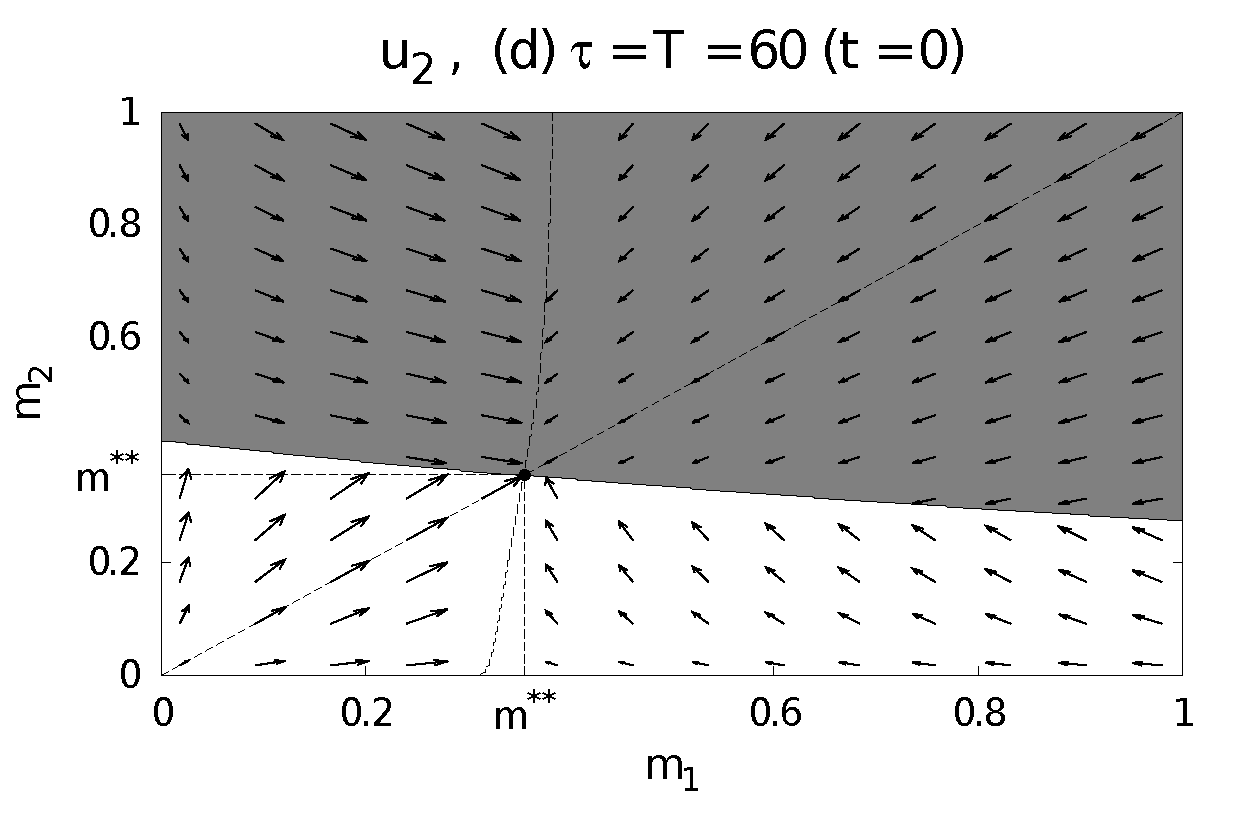
\includegraphics[width = 0.48 \textwidth]{figures/Figure_5d_2.pdf}
}
\bf \caption{\it In the white regions, the fungus enters spore production. In contrast in the gray, it enters mycelia production at a particular time instance. Also, the field corresponds to its velocity of production.
% Finite-difference approximations of the saddle feedback
% control strategies at several time instants. White and gray colors show the
% regions of the control values $ 0 $ and $ 1 ${\rm ,} respectively. Also
% illustrated are the fields of the corresponding forward-time velocities.
}
\label{Fig_5}
\end{figure}

Fig.~\ref{Fig_5} illustrates the appearance and time evolution of four
approximate switching curves. For $ \tau \geqslant \tau^{**} $, they intersect
at the point~$ \: \left( m^{**}, m^{**} \right) \, = \, 10^{-4}
\cdot \left( M^{**}, M^{**} \right) $. With the further increase of $ \tau $, the 
feedback control approaches a stationary form. There is less competition for resources between the fungi. Fig.~\ref{Fig_7}
is a three-dimensional graph of the 
four control switching surfaces (the fungi's direction to progress and avoid invasion). 
For $ \tau \geqslant \tau^{**} $, the point~$ \left( m^{**}, m^{**} \right) $
attracts forward-time trajectories. It determines a steady-state equilibrium
strategy for both cohorts. Simultaneously, one can interpret the four surfaces as necessary actions of the cohorts to avoid invasion.

%todo: describe what is happening in the figures
\begin{figure}
\center{ 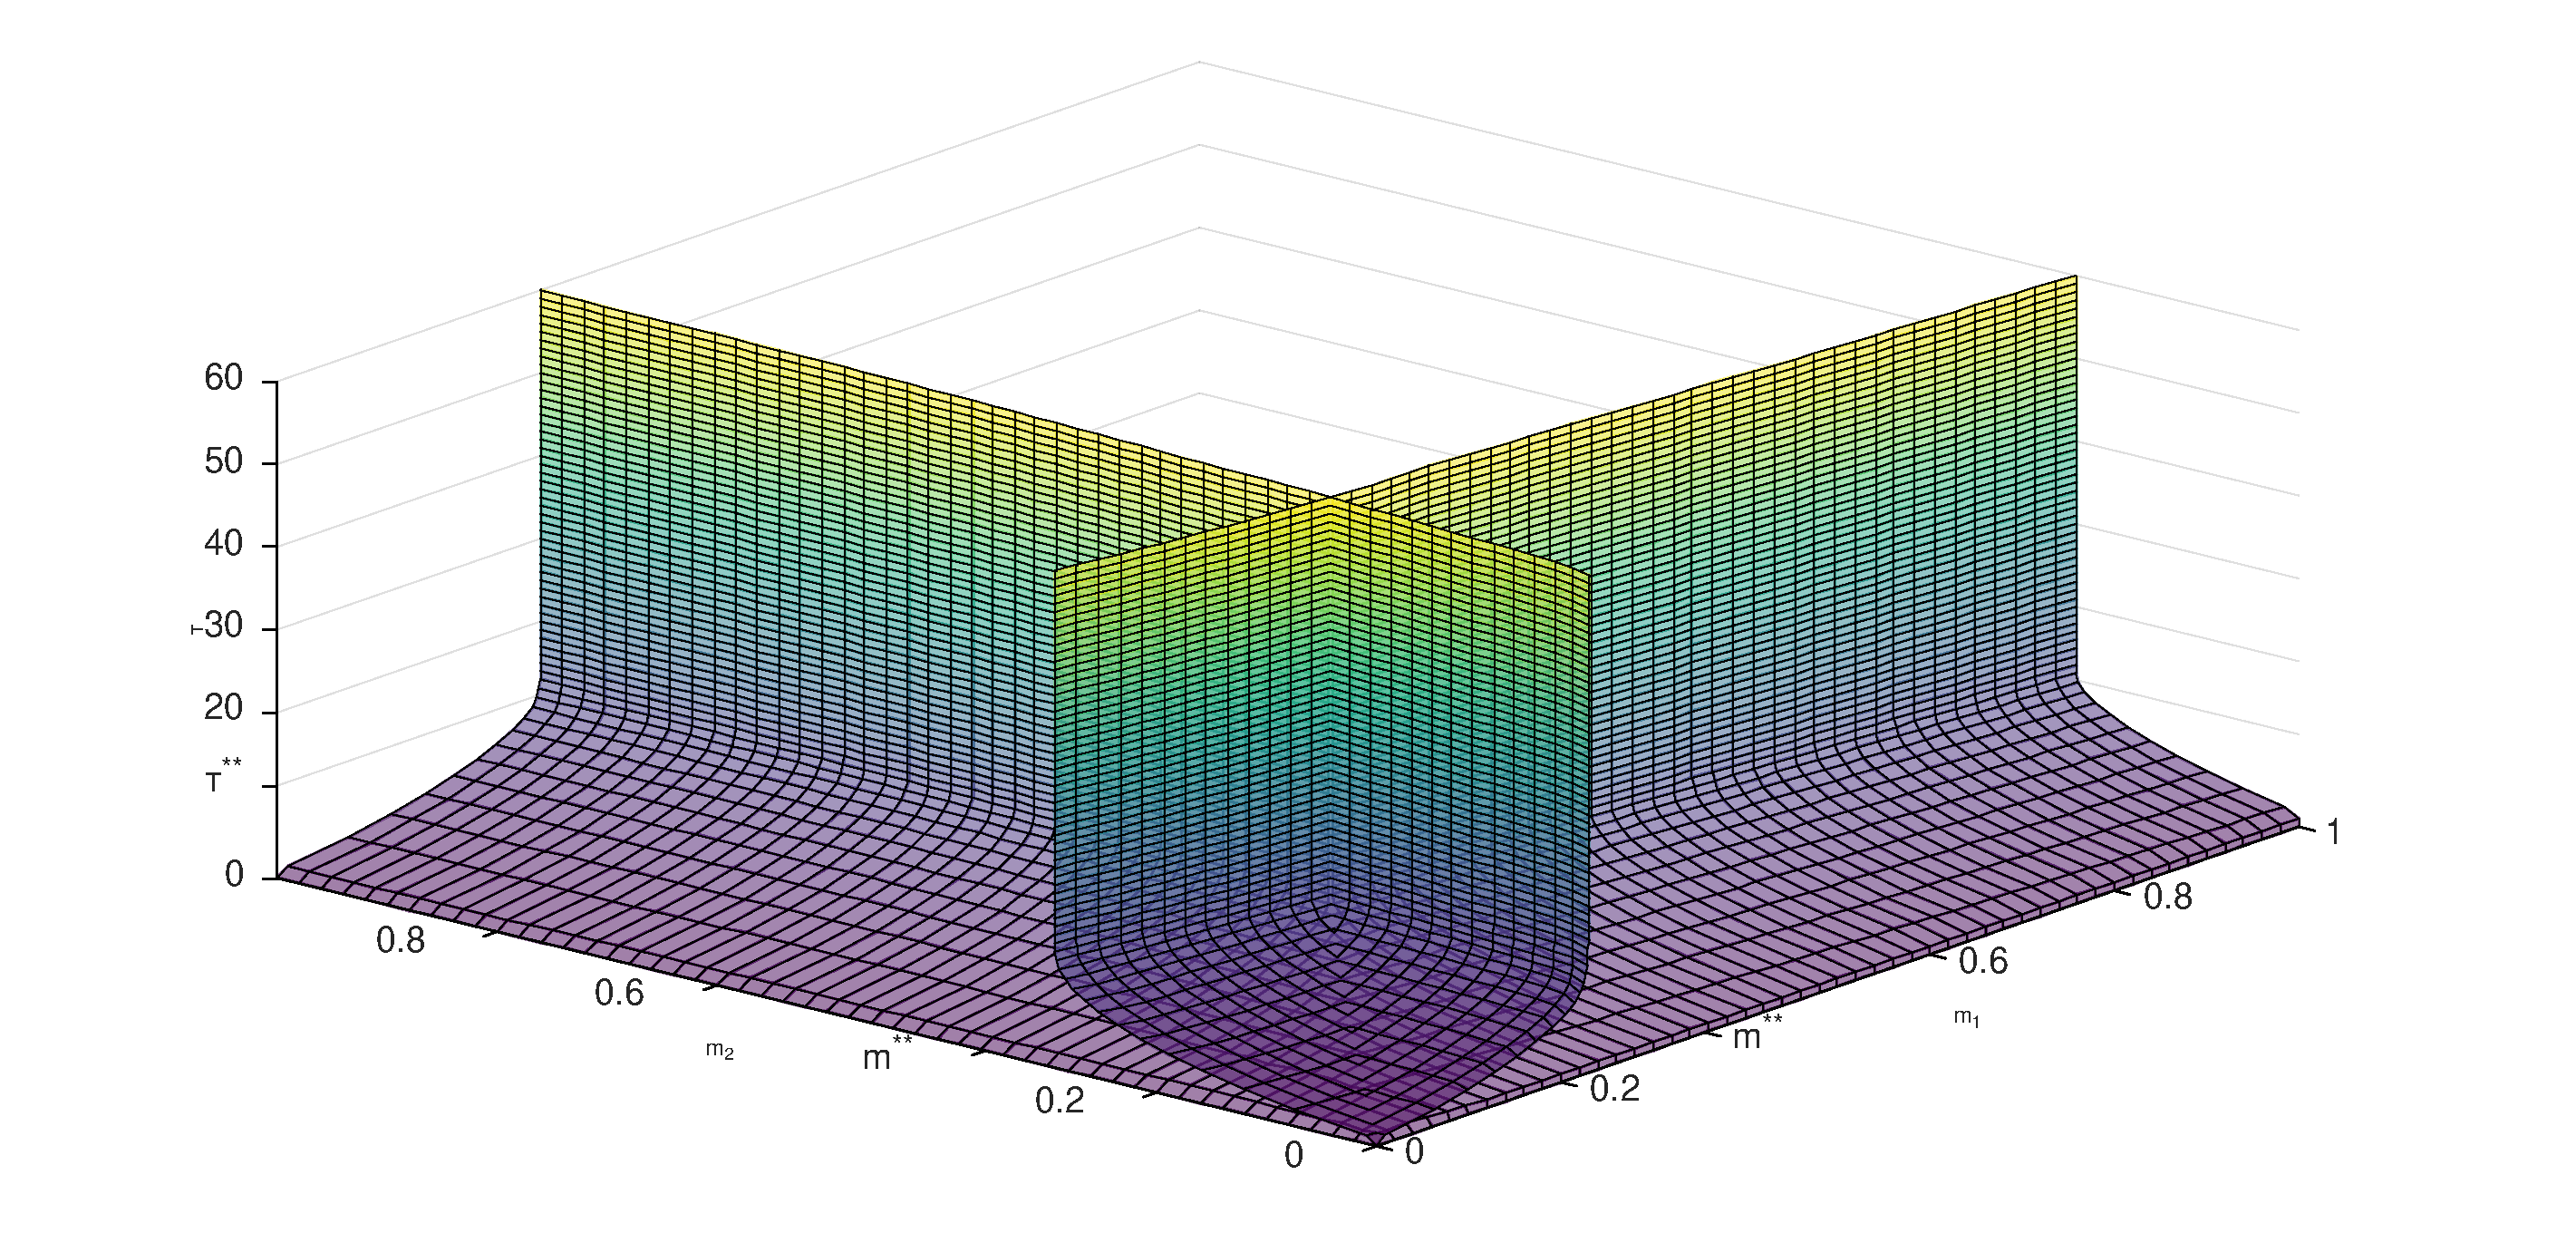
\includegraphics[width = 0.98 \textwidth]{figures/Figure_7.pdf} }
\bf \caption{\it The four control switching surfaces in the three-dimensional
space~$ (m_1, m_2, \tau) $.}
\label{Fig_7}
\end{figure}

From Fig.~{\rm \ref{Fig_4},} one can see that{\rm ,} in the considered domain
of initial states{\rm ,} the value $ V \left( 0, M_1^0, M_2^0 \right) $ of
the zero-sum feedback differential game is negative for $ M_1^0 > M_2^0 ${\rm ,}
zero for $ M_1^0 = M_2^0 ${\rm ,} and positive for $ M_1^0 < M_2^0 $. The strategy of cohort~{\rm 1} is uninvadable
if $ M_1^0 \geqslant M_2^0 $. Similarly{\rm ,} the strategy of cohort~{\rm 2} is uninvadable if $ M_1^0
\leqslant M_2^0 $. 


\section{Conclusion}
This report focuses on constructing a strategy for constructing benchmark resource allocation strategies. This paper also focuses on how differing pathogens might compete and allows us the ability to compare actual infection mechanisms.
We also focus solely on resource allocation equilibrium for the one-seasonal dynamics of two biotrophic fungal cohorts within a shared host plant. 

Though not mentioned in this paper, it is also relevant to investigate long-seasonal dynamics where the cohorts compete longer. Other relevant situations occur when the pathogens gain the ability to evolve, and the amount and spore-producing capacity, and when efficiencies of the pathogens begin to differ. Also interesting are situations where there are two separate and different species of fungi.

One may exploit specific discrete rules to
transition from one season to another \cite{MailleretLemesle2009,Akhmetzhanov2012}.
Another important research direction is to characterize such equilibria
themselves and whether they represent evolutionary attractors or not, and how the
situation may change through evolution.

\appendix

\section{Common terms}\label{terms}
\begin{enumerate}
    \item\label{term:zerosum} \textbf{Zero-sum feedback game}: a game in which one of the players wants the game to reach an open target (wants to take over, invade), while the want to avoid this target forever (prevent a takeover, defend)\cite{zerosumgame}.
    \item\label{term:pathogen} \textbf{Pathogen}: this is an infectious organism; this paper mostly discusses fungal invaders.
    \item\label{term:resident} \textbf{Resident pathogen}: this is the original organism, the first pathogen.
    \item\label{term:mutant} \textbf{Mutant pathogen}: this is a strain of the same species of the organism as the resident species but has a mutation through physical separation or natural mutation or otherwise.
    \item\label{term:mycelia} \textbf{Mycelia}: the ``roots'' of a fungus, made of extremely fine branches called hyphae. 
    \item\label{term:cohort} \textbf{Cohort}: typically means a person or thing that is typically on ``your side.'' This paper typically refers to a pathogen that belongs to the same species but differs slightly and is not of the same organism.
    \item\label{term:biotrohpic} \textbf{Biotrophic}: describes a parasite attached to a plant, a plant parasite. 
    \item\label{term:nutrientflux} \textbf{Nutrient flux}: the number of nutrients consumed by the pathogen.
    \item\label{term:differentialgame} \textbf{Differential game's value}:  the value of a function at a particular time when the function changes with time. 
    \item\label{term:marginal} \textbf{Two marginal fitness criteria}: a value or function that is wanting to be or altered or monitored, in this document, it is typically the spore production, and the mycelia production.
    \item\label{term:statevariables} \textbf{State Variables}: these are variables that set the equation or system stage and define the initial circumstances of the problem. These include items like lesion density or the rate of decay in the system.
    \item\label{term:saddlecontrol} \textbf{Saddle control strategies}: a function or system determining the saddle point of an equation.
    \item\label{term:carryingcapacity} \textbf{Carrying capacity}: the maximum size of a population that is sustainable in an environment.
    
\end{enumerate}
%%%%%%%%%%%%%%%%%%%%%%%%%%%%%%%%%%%%%%%%%%%%%%1
\section{Useful Mathematical Definitions}\label{mathdefs}
\begin{enumerate}
   % \item\label{math:jacobi} \textbf{Jacobi}
    \item\label{math:infimum} \textbf{Infimum}: the subset of the greatest elements in a set; the greatest lower bound \cite{infimumsupremum}.
    \item\label{math:supremum} \textbf{Supremum}: the subset of the least element that is greater than or equal to all S elements if such an element exists  \cite{infimumsupremum}.
    \item\label{math:Argmaxmin} \textbf{Arg max/Arg min}: a set of a function in which the values are maximized (Arg max) or minimized (Arg min).
    \item\label{math:saddlepoint} \textbf{Saddle point}: the point in which the slopes in all directions are zero, and the graph makes a saddle shape.
    \item\label{math:maximinminimax} \textbf{Maximin / Minimax}: the largest in a series of minima (maximin) or the smallest in a maxima series (minimax).
    %\item\label{math:valuefunction} \textbf{Value function}:
    \item\label{math:cauchyproblem} \textbf{Cauchy problem}: a problem that asks for a partial differential equation that satisfies certain conditions given by a hypersurface.
    \item\label{math:nonsmooth} \textbf{Non-smooth}: describes a non infinitely differential function.
    %%%%%%%%%%%%%%%%ask ivan
    \item\label{math:viscosity} \textbf{Viscosity solution}: a solution that is both a supersolution and a subsolution.
    \item\label{math:lipschitz} \textbf{Lipschitz continuous}: describing a function that has a limit on how fast it changes.
    \item\label{math:rademacher} \textbf{Rademacher's theorem}: Let $f: \mathbb{R} \rightarrow \mathbb{R} $ be any Lipschitz continuous function. Then $f$ is differentiable in almost anywhere $x \in \mathbb{R}^n$.
    \item\label{math:lebesgue} \textbf{Lebesgue measure}: a standard method of assigning a measure to a subset, a unit of measure.
    \item\label{math:monotone} \textbf{Monotone function}: A function that preserves order, a function that is always rising or decreasing. A function is monotonically increasing if for all $x$ and $y$ where $x \leq y$ then $f(x) \leq f(y)$, and reverse for monotonically decreasing.
    \item\label{math:diffusionproblem} \textbf{Numerical Diffusion Problems}: a difficulty that often arises when the computed medium differs from the actual medium, or it arises when it should not in the first place.
    %\item\label{math:pontryagin} \textbf{Pontryagin's maximum principle}:
\end{enumerate}

\section{}\label{appendix:references}
\begin{thebibliography}{}

\bibitem{YegorovGrognardMailleretHalkettBernhard2019}
I.~Yegorov, F.~Grognard, L.~Mailleret, F.~Halkett, P.~Bernhard. A dynamic game
approach to uninvadable strategies for biotrophic
pathogens. {\it Dynamic Games and Applications} 2020; {\bf 10}(1): 257--296.


\bibitem{ROCHJ2019}
Bokanowski,~O., Desilles,~A., Zidani,~H., and Zhao,~J.
User's guide for the ROC-HJ solver: Finite Differences and Semi-Lagrangian
methods. January~21,~2019. Version 2.5.4.
URL: \url{https://uma.ensta-paristech.fr/soft/ROC-HJ}

\bibitem{BernhardGrognardMailleretAkhmetzhanov2010}
Bernhard,~P., Grognard,~F., Mailleret,~L., and Akhmetzhanov,~A.
ESS for life-history traits of cooperating consumers facing cheating mutants.
[Research Report] RR--7314, INRIA, 2010.
URL: \url{https://hal.inria.fr/inria-00491489v2}

\bibitem{DercoleRinaldi2008}
Dercole,~F. and Rinaldi,~S.
{\it Analysis of Evolutionary Processes{\rm :} The Adaptive Dynamics Approach
and Its Applications}.
Princeton University Press: Princeton, 2008.

\bibitem{FlemingSoner2006}
Fleming,~W.\,H. and Soner,~H.\,M.
{\it Controlled Markov Processes and Viscosity Solutions}.
Springer-Verlag: New York, 2006.

\bibitem{Subbotin1995}
Subbotin,~A.\,I.
{\it Generalized Solutions of First-Order PDEs{\rm :} The Dynamical
Optimization Perspective}.
Birkhauser: Boston, 1995.

\bibitem{BotkinHoffmannTurova2011}
Botkin,~N.\,D., Hoffmann,~K.-H., and Turova,~V.-L.
Stable numerical schemes for solving Hamilton--Jacobi--Bellman--Isaacs
equations.
{\it SIAM Journal on Scientific Computing} 2011; {\bf 33}(2): 992--1007.

\bibitem{OsherShu1991}
Osher,~S. and Shu,~C.-W. High order essentially non-oscillatory schemes for
Hamilton--Jacobi equations.
{\it SIAM Journal on Numerical Analysis} 1991; {\bf 28}(4): 907--922.

\bibitem{BokanForcadelZidani2010}
Bokanowski,~O., Forcadel,~N., and Zidani,~H.
Reachability and minimal times for state constrained nonlinear problems without
any controllability assumption.
{\it SIAM Journal on Control and Optimization} 2010; {\bf 48}: 4292--4316.

\bibitem{PressTeukolskyVetterlingFlannery2007}
Press,~W.\,H., Teukolsky,~S.\,A., Vetterling,~W.\,T., and Flannery,~B.\,P.
{\it Numerical Recipes{\rm :} The Art of Scientific Computing}. Cambridge
University Press: New~York, 2007.

\bibitem{Yong2015}
Yong,~J.
{\it Differential Games{\rm :} A Concise Introduction}.
World Scientific Publishing: Singapore, 2015.

\bibitem{MailleretLemesle2009}
Mailleret,~L. and Lemesle,~V.
A note on semi-discrete modelling in life sciences.
{\it Philosophical Transactions of the Royal Society A} 2009; {\bf 367}:
4779--4799.

\bibitem{Akhmetzhanov2012}
Akhmetzhanov,~A.\,R., Grognard,~F., Mailleret,~L., and Bernhard,~P.
Join forces or cheat: Evolutionary analysis of a consumer-resource system.
In {\it Advances in Dynamic Games{\rm ,}
Volume {\rm 12} of the series Annals of the International Society of Dynamic
Games}, 73--95.
Springer: New York, 2012.

\bibitem{YegorovGrognardMailleretHalkett2017}
Yegorov,~I., Grognard,~F., Mailleret,~L., Halkett,~F.
Optimal resource allocation for biotrophic plant
pathogens.
IFAC-PapersOnline 50(1):3154–3159.

\bibitem{data_ivan.h}
\raggedright Glasford, S., Yegorov, I. \textit{\texttt{data\_*.h} used by
ROC-HJ to set the problem statement.}
\url{https://raw.githubusercontent.com/stevenglasford/Seminar_NDSU_2020/main/ivan_to_2.5/data/data_user_biotroph_fungi_game.h}

\bibitem{infimumsupremum}
Rudin, Walter (1976). ""Chapter 1 The Real and Complex Number Systems"". Principles of Mathematical Analysis ("print") (3rd ed.). McGraw-Hill. p. 4. ISBN 0-07-054235-X.

\bibitem{zerosumgame}
Cardaliaguet P., Rainer C. (2016) Zero-Sum Differential Games. In: Basar T., Zaccour G. (eds) Handbook of Dynamic Game Theory. Springer, Cham. https://doi.org/10.1007/978-3-319-27335-8\_4-1

\bibitem{cauchy}
Jacques Hadamard (1923), Lectures on Cauchy's Problem in Linear Partial Differential Equations, Dover Phoenix editions

\end{thebibliography}

\section{Code Snippets}

\begin{figure}[h]
    \inputminted[
        frame=lines,
        framesep=2mm,
        baselinestretch=1.2,
        fontsize=\footnotesize,
        firstline=15, 
        lastline=17]{c}{code/data.h}
\caption{A few configuration variables are needed to solve the equation using ROC-HJ, MFD being the monotone finite difference method.}
\label{code:defaults}
\end{figure}

\begin{figure}[h]
    \centering
    \inputminted[frame=lines,
        framesep=2mm,
        baselinestretch=1.2,
        fontsize=\footnotesize,
        firstline=137, 
        lastline=151]{c}{code/data.h}
    \caption{Function in C++ written for ROC-HJ describing the distributed
             cost equation.}
    \label{code:cost}
\end{figure}

\begin{figure}[h]
    \centering
    \inputminted[frame=lines,
        framesep=2mm,
        baselinestretch=1.2,
        fontsize=\footnotesize,
        firstline=120, 
        lastline=135]{c}{code/data.h}
    \caption{A C++ function for use by ROC-HJ to describe the required
             dynamic equation.}
    \label{code:dynamic}
\end{figure}

\hspace{1in}

\noindent


\end{document}
